\documentclass[]{article}
\usepackage{lmodern}
\usepackage{amssymb,amsmath}
\usepackage{ifxetex,ifluatex}
\usepackage{fixltx2e} % provides \textsubscript
\ifnum 0\ifxetex 1\fi\ifluatex 1\fi=0 % if pdftex
  \usepackage[T1]{fontenc}
  \usepackage[utf8]{inputenc}
\else % if luatex or xelatex
  \ifxetex
    \usepackage{mathspec}
  \else
    \usepackage{fontspec}
  \fi
  \defaultfontfeatures{Ligatures=TeX,Scale=MatchLowercase}
\fi
% use upquote if available, for straight quotes in verbatim environments
\IfFileExists{upquote.sty}{\usepackage{upquote}}{}
% use microtype if available
\IfFileExists{microtype.sty}{%
\usepackage{microtype}
\UseMicrotypeSet[protrusion]{basicmath} % disable protrusion for tt fonts
}{}
\usepackage[margin=1in]{geometry}
\usepackage{hyperref}
\hypersetup{unicode=true,
            pdftitle={Template for writing scientific papers in R markdown},
            pdfauthor={Petr Keil, pkeil@seznam.cz, modified by Simon Knight, sjgknight@gmail.com},
            pdfborder={0 0 0},
            breaklinks=true}
\urlstyle{same}  % don't use monospace font for urls
\usepackage{color}
\usepackage{fancyvrb}
\newcommand{\VerbBar}{|}
\newcommand{\VERB}{\Verb[commandchars=\\\{\}]}
\DefineVerbatimEnvironment{Highlighting}{Verbatim}{commandchars=\\\{\}}
% Add ',fontsize=\small' for more characters per line
\usepackage{framed}
\definecolor{shadecolor}{RGB}{248,248,248}
\newenvironment{Shaded}{\begin{snugshade}}{\end{snugshade}}
\newcommand{\AlertTok}[1]{\textcolor[rgb]{0.94,0.16,0.16}{#1}}
\newcommand{\AnnotationTok}[1]{\textcolor[rgb]{0.56,0.35,0.01}{\textbf{\textit{#1}}}}
\newcommand{\AttributeTok}[1]{\textcolor[rgb]{0.77,0.63,0.00}{#1}}
\newcommand{\BaseNTok}[1]{\textcolor[rgb]{0.00,0.00,0.81}{#1}}
\newcommand{\BuiltInTok}[1]{#1}
\newcommand{\CharTok}[1]{\textcolor[rgb]{0.31,0.60,0.02}{#1}}
\newcommand{\CommentTok}[1]{\textcolor[rgb]{0.56,0.35,0.01}{\textit{#1}}}
\newcommand{\CommentVarTok}[1]{\textcolor[rgb]{0.56,0.35,0.01}{\textbf{\textit{#1}}}}
\newcommand{\ConstantTok}[1]{\textcolor[rgb]{0.00,0.00,0.00}{#1}}
\newcommand{\ControlFlowTok}[1]{\textcolor[rgb]{0.13,0.29,0.53}{\textbf{#1}}}
\newcommand{\DataTypeTok}[1]{\textcolor[rgb]{0.13,0.29,0.53}{#1}}
\newcommand{\DecValTok}[1]{\textcolor[rgb]{0.00,0.00,0.81}{#1}}
\newcommand{\DocumentationTok}[1]{\textcolor[rgb]{0.56,0.35,0.01}{\textbf{\textit{#1}}}}
\newcommand{\ErrorTok}[1]{\textcolor[rgb]{0.64,0.00,0.00}{\textbf{#1}}}
\newcommand{\ExtensionTok}[1]{#1}
\newcommand{\FloatTok}[1]{\textcolor[rgb]{0.00,0.00,0.81}{#1}}
\newcommand{\FunctionTok}[1]{\textcolor[rgb]{0.00,0.00,0.00}{#1}}
\newcommand{\ImportTok}[1]{#1}
\newcommand{\InformationTok}[1]{\textcolor[rgb]{0.56,0.35,0.01}{\textbf{\textit{#1}}}}
\newcommand{\KeywordTok}[1]{\textcolor[rgb]{0.13,0.29,0.53}{\textbf{#1}}}
\newcommand{\NormalTok}[1]{#1}
\newcommand{\OperatorTok}[1]{\textcolor[rgb]{0.81,0.36,0.00}{\textbf{#1}}}
\newcommand{\OtherTok}[1]{\textcolor[rgb]{0.56,0.35,0.01}{#1}}
\newcommand{\PreprocessorTok}[1]{\textcolor[rgb]{0.56,0.35,0.01}{\textit{#1}}}
\newcommand{\RegionMarkerTok}[1]{#1}
\newcommand{\SpecialCharTok}[1]{\textcolor[rgb]{0.00,0.00,0.00}{#1}}
\newcommand{\SpecialStringTok}[1]{\textcolor[rgb]{0.31,0.60,0.02}{#1}}
\newcommand{\StringTok}[1]{\textcolor[rgb]{0.31,0.60,0.02}{#1}}
\newcommand{\VariableTok}[1]{\textcolor[rgb]{0.00,0.00,0.00}{#1}}
\newcommand{\VerbatimStringTok}[1]{\textcolor[rgb]{0.31,0.60,0.02}{#1}}
\newcommand{\WarningTok}[1]{\textcolor[rgb]{0.56,0.35,0.01}{\textbf{\textit{#1}}}}
\usepackage{longtable,booktabs}
\usepackage{graphicx,grffile}
\makeatletter
\def\maxwidth{\ifdim\Gin@nat@width>\linewidth\linewidth\else\Gin@nat@width\fi}
\def\maxheight{\ifdim\Gin@nat@height>\textheight\textheight\else\Gin@nat@height\fi}
\makeatother
% Scale images if necessary, so that they will not overflow the page
% margins by default, and it is still possible to overwrite the defaults
% using explicit options in \includegraphics[width, height, ...]{}
\setkeys{Gin}{width=\maxwidth,height=\maxheight,keepaspectratio}
\IfFileExists{parskip.sty}{%
\usepackage{parskip}
}{% else
\setlength{\parindent}{0pt}
\setlength{\parskip}{6pt plus 2pt minus 1pt}
}
\setlength{\emergencystretch}{3em}  % prevent overfull lines
\providecommand{\tightlist}{%
  \setlength{\itemsep}{0pt}\setlength{\parskip}{0pt}}
\setcounter{secnumdepth}{5}
% Redefines (sub)paragraphs to behave more like sections
\ifx\paragraph\undefined\else
\let\oldparagraph\paragraph
\renewcommand{\paragraph}[1]{\oldparagraph{#1}\mbox{}}
\fi
\ifx\subparagraph\undefined\else
\let\oldsubparagraph\subparagraph
\renewcommand{\subparagraph}[1]{\oldsubparagraph{#1}\mbox{}}
\fi

%%% Use protect on footnotes to avoid problems with footnotes in titles
\let\rmarkdownfootnote\footnote%
\def\footnote{\protect\rmarkdownfootnote}

%%% Change title format to be more compact
\usepackage{titling}

% Create subtitle command for use in maketitle
\providecommand{\subtitle}[1]{
  \posttitle{
    \begin{center}\large#1\end{center}
    }
}

\setlength{\droptitle}{-2em}

  \title{Template for writing scientific papers in R markdown}
    \pretitle{\vspace{\droptitle}\centering\huge}
  \posttitle{\par}
    \author{Petr Keil, \href{mailto:pkeil@seznam.cz}{\nolinkurl{pkeil@seznam.cz}},
modified by Simon Knight,
\href{mailto:sjgknight@gmail.com}{\nolinkurl{sjgknight@gmail.com}}}
    \preauthor{\centering\large\emph}
  \postauthor{\par}
      \predate{\centering\large\emph}
  \postdate{\par}
    \date{11/1/2015, and March 2018}


\begin{document}
\maketitle

\hypertarget{preliminaries}{%
\section{Preliminaries}\label{preliminaries}}

Load packages. If you don't have them installed already, you should
uncomment (delete the \#) the first 3 lines (starting
`install.packages', and `devtools')

Once you've done that, you can test the file by using the `knit' button
(just above this code chunk).

Read more about R markdown and `kniting' (rendering) documents
\url{https://rmarkdown.rstudio.com/authoring_quick_tour.html\#overview}

First, we'll load some packages

\begin{Shaded}
\begin{Highlighting}[]
\CommentTok{#install.packages(c("tidyverse","flexdashboard","shiny","knitcitations","bibtex","psych","devtools","curl","reshape2","tidyr","lattice","kfigr","rwunderground","gganimate"))}
\CommentTok{# devtools::install_github("cboettig/knitcitations")}
\CommentTok{#devtools::install_github("benmarwick/wordcountaddin", type = "source", dependencies = TRUE)}
\CommentTok{#go to Tools > Addins to select the wordcountaddin }

  \KeywordTok{library}\NormalTok{(knitcitations); }\KeywordTok{cleanbib}\NormalTok{()}
\end{Highlighting}
\end{Shaded}

\begin{verbatim}
## Warning: package 'knitcitations' was built under R version 3.5.2
\end{verbatim}

\begin{Shaded}
\begin{Highlighting}[]
  \KeywordTok{cite_options}\NormalTok{(}\DataTypeTok{citation_format =} \StringTok{"pandoc"}\NormalTok{, }\DataTypeTok{check.entries=}\OtherTok{FALSE}\NormalTok{)}
  \KeywordTok{library}\NormalTok{(bibtex)}
\end{Highlighting}
\end{Shaded}

\begin{verbatim}
## Warning: package 'bibtex' was built under R version 3.5.3
\end{verbatim}

\begin{Shaded}
\begin{Highlighting}[]
  \KeywordTok{library}\NormalTok{(psych)}
\end{Highlighting}
\end{Shaded}

\begin{verbatim}
## Warning: package 'psych' was built under R version 3.5.2
\end{verbatim}

\begin{Shaded}
\begin{Highlighting}[]
  \KeywordTok{library}\NormalTok{(curl)}
\end{Highlighting}
\end{Shaded}

\begin{verbatim}
## Warning: package 'curl' was built under R version 3.5.3
\end{verbatim}

\begin{Shaded}
\begin{Highlighting}[]
  \KeywordTok{library}\NormalTok{(devtools)}
\end{Highlighting}
\end{Shaded}

\begin{verbatim}
## Warning: package 'devtools' was built under R version 3.5.2
\end{verbatim}

\begin{verbatim}
## Warning: package 'usethis' was built under R version 3.5.3
\end{verbatim}

\begin{Shaded}
\begin{Highlighting}[]
  \KeywordTok{library}\NormalTok{(dplyr)}
\end{Highlighting}
\end{Shaded}

\begin{verbatim}
## Warning: package 'dplyr' was built under R version 3.5.3
\end{verbatim}

\begin{verbatim}
## 
## Attaching package: 'dplyr'
\end{verbatim}

\begin{verbatim}
## The following objects are masked from 'package:stats':
## 
##     filter, lag
\end{verbatim}

\begin{verbatim}
## The following objects are masked from 'package:base':
## 
##     intersect, setdiff, setequal, union
\end{verbatim}

\begin{Shaded}
\begin{Highlighting}[]
  \KeywordTok{library}\NormalTok{(ggplot2)}
\end{Highlighting}
\end{Shaded}

\begin{verbatim}
## Warning: package 'ggplot2' was built under R version 3.5.3
\end{verbatim}

\begin{verbatim}
## 
## Attaching package: 'ggplot2'
\end{verbatim}

\begin{verbatim}
## The following objects are masked from 'package:psych':
## 
##     %+%, alpha
\end{verbatim}

\begin{Shaded}
\begin{Highlighting}[]
  \KeywordTok{library}\NormalTok{(psych)}
  \KeywordTok{library}\NormalTok{(tidyr)}
\end{Highlighting}
\end{Shaded}

\begin{verbatim}
## Warning: package 'tidyr' was built under R version 3.5.2
\end{verbatim}

\begin{Shaded}
\begin{Highlighting}[]
  \KeywordTok{library}\NormalTok{(reshape2)}
\end{Highlighting}
\end{Shaded}

\begin{verbatim}
## Warning: package 'reshape2' was built under R version 3.5.2
\end{verbatim}

\begin{verbatim}
## 
## Attaching package: 'reshape2'
\end{verbatim}

\begin{verbatim}
## The following object is masked from 'package:tidyr':
## 
##     smiths
\end{verbatim}

\begin{Shaded}
\begin{Highlighting}[]
  \KeywordTok{library}\NormalTok{(knitr)}
  \KeywordTok{library}\NormalTok{(lattice) }\CommentTok{#just to illustrate another histogram function}
\end{Highlighting}
\end{Shaded}

\begin{verbatim}
## Warning: package 'lattice' was built under R version 3.5.2
\end{verbatim}

\begin{Shaded}
\begin{Highlighting}[]
  \KeywordTok{library}\NormalTok{(kfigr) }\CommentTok{#this lets us crossreference figures, etc. Read more about it https://github.com/mkoohafkan/kfigr/edit/master/vignettes/introduction.Rmd }
\end{Highlighting}
\end{Shaded}

\begin{verbatim}
## Warning: package 'kfigr' was built under R version 3.5.2
\end{verbatim}

\begin{verbatim}
## knitr hook "anchor" is now available
\end{verbatim}

\begin{Shaded}
\begin{Highlighting}[]
  \KeywordTok{options}\NormalTok{(}\StringTok{"kfigr.prefix"}\NormalTok{ =}\StringTok{ }\OtherTok{TRUE}\NormalTok{)}
  \KeywordTok{options}\NormalTok{(}\StringTok{"kfigr.link"}\NormalTok{ =}\StringTok{ }\OtherTok{TRUE}\NormalTok{)}
\end{Highlighting}
\end{Shaded}

If you want to get your own weather data, you can uncomment the below

\begin{Shaded}
\begin{Highlighting}[]
\CommentTok{#    library(rwunderground) #see https://github.com/ALShum/rwunderground - you'll need to register an api key}
\CommentTok{#source("C:\textbackslash{}\textbackslash{}Users\textbackslash{}\textbackslash{}125295_admin\textbackslash{}\textbackslash{}Oxygen Enterprise\textbackslash{}\textbackslash{}Project data\textbackslash{}\textbackslash{}RProjects\textbackslash{}\textbackslash{}DSI\textbackslash{}\textbackslash{}rwunderground_key.R") #this loads my key without making it visible to you . That file just has one line: }
  \CommentTok{#rwunderground::set_api_key("mykey")}
\end{Highlighting}
\end{Shaded}

\hypertarget{abstract-not-necessary-for-at2}{%
\section{Abstract (not necessary for
AT2)}\label{abstract-not-necessary-for-at2}}

\emph{Please note that while we're keen for you to extend your technical
skills, \emph{a key concern of AT2 is how you communicate about and with
data}, so \emph{take caution not to get distracted by technical issues,
and to focus on the criteria}. This template mirrors the Word file to
provide a structure for the report. Make sure that you read it closely,
several times.}

\hypertarget{word-length}{%
\section{Word Length}\label{word-length}}

2800 words (excluding data excerpts and appendices, visualisations, and
references) To check this, you can either copy the html output to word,
or use the addin Word Count Addin. E.g.
\texttt{wordcountaddin:::text\_stats()}

\begin{Shaded}
\begin{Highlighting}[]
\NormalTok{wordcountaddin}\OperatorTok{:::}\KeywordTok{text_stats}\NormalTok{()}
\end{Highlighting}
\end{Shaded}

\begin{verbatim}
## 
## Attaching package: 'sylly'
\end{verbatim}

\begin{verbatim}
## The following object is masked from 'package:psych':
## 
##     describe
\end{verbatim}

\begin{verbatim}
## For information on available language packages for 'koRpus', run
## 
##   available.koRpus.lang()
## 
## and see ?install.koRpus.lang()
\end{verbatim}

\begin{longtable}[]{@{}lll@{}}
\toprule
Method & koRpus & stringi\tabularnewline
\midrule
\endhead
Word count & 1652 & 1607\tabularnewline
Character count & 9334 & 9276\tabularnewline
Sentence count & 105 & Not available\tabularnewline
Reading time & 8.3 minutes & 8 minutes\tabularnewline
\bottomrule
\end{longtable}

\hypertarget{using-this-template}{%
\section{Using this template}\label{using-this-template}}

This is the suggested structure for your report. The basic structure is
similar to the style of academic papers and, if followed, should ensure
that everything you need to include is present. I have included the
assessment criteria at the relevant places to remind you of what needs
to be in the report.

You are free to vary the structure by renaming the sections, including
other sections, or dropping ones that you don't use. Keep in mind that
the suggested structure is conventional (and therefore easy to follow),
practical, and comprehensive. (Criterion 5: Professionally presented in
a manner appropriate to the discipline.) If you do use this template,
you will need to install R, RStudio, and the packages listed in the code
block at the head of this document.

Note: We have provided some sample code below, along with some text
between angle brackets, \textless{} \textgreater. All of this should be
replaced by your work.

\textbf{\emph{Please don't forget to include a title, name, student
number, etc. on a covering sheet}}

\hypertarget{introduction}{%
\section{Introduction}\label{introduction}}

\textless a paragraph that gives an overview of what you've
done\textgreater{}

\hypertarget{citations}{%
\subsection{Citations}\label{citations}}

You'll want to ensure that you connect what you did, and what you found,
to the wider context of data science - including external sources of
information (such as academic studies). You can build your reflection
(criterion 4) through the paper like that. You'll need to work out how
to cite\ldots{}

\hypertarget{using-dois}{%
\subsubsection{Using DOIs}\label{using-dois}}

Use: * \texttt{citet} if you want an inline citation, like Knight (2019)
says * and \texttt{citep} if you want it in brackets (Knight, 2019)

The relationship was first described by Halpern \emph{et al.} (2006).
However, there are also opinions that the relationship is spurious (Keil
\emph{et al.} 2012).

\hypertarget{using-urls}{%
\subsubsection{Using URLs}\label{using-urls}}

Sometimes you can use the URL to cite: (Knight \& Shum 2020) although
this service may be down at the moment.

\hypertarget{citing-using-a-.bib-file-and-citation-manager}{%
\subsubsection{Citing using a .bib file and citation
manager}\label{citing-using-a-.bib-file-and-citation-manager}}

If you create a .bib file, you can cite using (Halpern \emph{et al.}
2006) - where your bib file has the `key' (the bit after the @) with all
the other detail. See the sample file!

\hypertarget{citing-packages}{%
\subsubsection{Citing packages}\label{citing-packages}}

Packages you use have their own citation function! So here, we're going
to cite R, and then knitcitations:

We used R for our calculations (R Core Team 2018), and we used package
\texttt{knitcitations} (Boettiger 2017) to make the bibliography.

\hypertarget{using-footnotes---a-good-option-especially-if-you-get-stuck-with-the-others}{%
\subsubsection{Using footnotes - a good option especially if you get
stuck with the
others!}\label{using-footnotes---a-good-option-especially-if-you-get-stuck-with-the-others}}

If you're stuck we'll just accept footnotes for this assignment (which
don't need the .bib or .csl or citep code). To insert them you just type
\texttt{\^{}{[}This\ is\ a\ footnote.{]}}, you'll get a hyperlinked
number and at the end of your document the list is automatically
created! Pretty useful right?\footnote{This is a footnote, see how it
  auto appears at the end of the doc.}

\hypertarget{putting-it-all-together}{%
\subsubsection{Putting it all together}\label{putting-it-all-together}}

The CSL file tells R how to format the citations. And the .bib file
includes other references - you can generate one of those from
Zotero/Mendeley/Endnote, etc. You can see the sample files with the
download folder (and just use the CSL file as it is).

\hypertarget{including-quotations}{%
\subsubsection{Including quotations}\label{including-quotations}}

\begin{quote}
This is a block quotation, if you have a long quote from someone this is
the best way to do it (but don't forget hte citation). This is a very
long line that will still be quoted properly when it wraps. Oh boy let's
keep writing to make sure this is long enough to actually wrap for
everyone. Oh, you can \emph{put} \textbf{Markdown} into a blockquote.
\end{quote}

\hypertarget{other-formatting}{%
\subsection{Other formatting}\label{other-formatting}}

You'll see that we can:

\begin{enumerate}
\def\labelenumi{\arabic{enumi}.}
\tightlist
\item
  Format things, e.g.
\end{enumerate}

\begin{itemize}
\item
  \emph{italicise}
\item
  \textbf{or bold}
\item
  \textbf{\emph{or even bold italics}} (you can also have numbered
  sublists\ldots)

  \ldots See the cheatsheet
  \url{https://rmarkdown.rstudio.com/authoring_basics.html} for more on
  this\ldots.to link to that by the way
  \href{https://rmarkdown.rstudio.com/authoring_basics.html}{I could
  have done this}
\end{itemize}

\begin{enumerate}
\def\labelenumi{\arabic{enumi}.}
\setcounter{enumi}{1}
\tightlist
\item
  And add headings using a \# (but note, to get that to display properly
  I had to `escape' it using a preceding backslash)
\item
  And we can use citation, inline code, and charts
\item
  All this means we can write a document, but we can also pull data in
  \emph{live} and display it to the reader, who can also download this
  Rmd to see how we did it\ldots it's pretty cool hey?
\end{enumerate}

But, just because it's in a different format, that doesn't mean you can
get away with not following normal writing conventions. Writing should
be in paragraphs, with correct spelling and grammar, and figures, etc.
should be fully explained to the reader. For example, it's weird that
I've just dumped Fig.1 image below, so in the methods, I'll make sure to
explain them properly. (Note though, that this does illustrate how to
include images - so if you do analysis outside R, you can still include
figures, etc. without the code being R based)

\begin{figure}
\centering
\includegraphics{https://github.com/adam-p/markdown-here/raw/master/src/common/images/icon48.png}
\caption{Fig.1 A random logo image}
\end{figure}

\hypertarget{description-of-process-or-method}{%
\section{Description of process, or
method}\label{description-of-process-or-method}}

\textless this is where you give details about what you've been
collecting and how much you data have; why you choose this data to
collect; how you managed the quality and frequency of collection issues;
what you did to anonymise or de-identify the data, and how you dealt
with the storage and sharing of data within the group. Do not include a
dump of all your data here. If you wish to include examples of data (and
I think you should) then put these in an appendix to the report.\\
Criterion 1: Justifies a method to obtain data from multiple sources,
for gaining insight into a chosen problem, including analysis of data
quality issues in the individual and group data.\textgreater{}

\hypertarget{analysis}{%
\section{Analysis}\label{analysis}}

\textless describe how you analysed your data, and how you contrasted
your data with the group's data.\\
Criterion 2: Justifies the analysis of the obtained data, including
quality issues, to draw conclusions in a professional and engaging
manner.\textgreater{}

\hypertarget{equations-probably-not-useful-but-just-in-case}{%
\subsection{Equations (probably not useful, but just in
case)}\label{equations-probably-not-useful-but-just-in-case}}

If you want to insert equations (you probably don't) you can do so using
the syntax below. You can also insert bits of inline code like, so the
\texttt{2+2} here is produced by a piece of code, and the 4 is produced
by an equation (namely \texttt{2+2})

The determinisstic part of the model is defined by this \textbf{in-line
equation} as \(\mu_i = \beta_0 + \beta_1x\), and the stochastic part by
the \textbf{centered equation}:

\[ \frac{1}{\sqrt{2\pi}\sigma}e^{-(x-\mu_i)^2/(2\sigma^2)} \]

\hypertarget{some-example-analysis-get-and-load-data}{%
\subsection{Some example analysis: Get and load
data}\label{some-example-analysis-get-and-load-data}}

If you downloaded the full folder, then the csv files you need are
there. You can also get your own weather data if you want.

\begin{Shaded}
\begin{Highlighting}[]
\CommentTok{# Sydney is 33.8688° S, 151.2093° E}
\CommentTok{#see https://github.com/ALShum/rwunderground - you'll need to register an api key}
\CommentTok{#use_metric = TRUE}

\NormalTok{end_date <-}\StringTok{ }\KeywordTok{Sys.Date}\NormalTok{()}\OperatorTok{-}\DecValTok{1}
\NormalTok{start_date <-}\StringTok{ }\KeywordTok{Sys.Date}\NormalTok{()}\OperatorTok{-}\DecValTok{35}

\CommentTok{#lookup_airport("Melbourne")}
\CommentTok{#set_location(zip_code = "2016") you can also use this}

\CommentTok{#weather_sydney <- history_range(set_location(airport_code = "SYD"), date_start = start_date, date_end = end_date, limit = 10, no_api = FALSE, use_metric = TRUE, key = get_api_key(), raw = FALSE, message = TRUE)}
\CommentTok{#write.csv(weather_sydney, file = "syd_weath.csv")}
\NormalTok{weather_sydney <-}\StringTok{ }\KeywordTok{read.csv}\NormalTok{(}\StringTok{"syd_weath.csv"}\NormalTok{, }\DataTypeTok{stringsAsFactors =}\NormalTok{ F)}

\CommentTok{#weather_melbourne <- history_range(set_location(PWS_id = "IVICTORI842"), date_start = start_date, date_end = end_date, limit = 10, no_api = FALSE, use_metric = TRUE, key = get_api_key(), raw = FALSE, message = TRUE) #deliberately taking data from a slightly worse station. Use airport_code = "YMML" for equiv}
\CommentTok{#weather_melbourne_gd <- history_range(set_location(PWS_id = "INORTHCO3"), date_start = start_date, date_end = end_date, limit = 10, no_api = FALSE, use_metric = TRUE, key = get_api_key(), raw = FALSE, message = TRUE)}
\CommentTok{#write.csv(weather_melbourne, file = "mel_weath.csv")}
\NormalTok{weather_melbourne <-}\StringTok{ }\KeywordTok{read.csv}\NormalTok{(}\StringTok{"mel_weath.csv"}\NormalTok{, }\DataTypeTok{stringsAsFactors =}\NormalTok{ F)}

\CommentTok{#to make this more interesting I'm going to randomly delete 500 observations}
\NormalTok{weather_melbourne <-}\StringTok{ }\NormalTok{weather_melbourne[}\OperatorTok{-}\KeywordTok{sample}\NormalTok{(}\DecValTok{1}\OperatorTok{:}\KeywordTok{nrow}\NormalTok{(weather_melbourne), }\DecValTok{800}\NormalTok{), ]}
\CommentTok{#for another 250 observations we're going to deliberately add noisy missing data in the form of -9999 values}
\NormalTok{weather_melbourne}\OperatorTok{$}\NormalTok{temp[}\KeywordTok{sample}\NormalTok{(}\KeywordTok{nrow}\NormalTok{(weather_melbourne),}\DecValTok{250}\NormalTok{)] <-}\StringTok{ }\DecValTok{-9999}

\CommentTok{#weather_sydney_summary <- history_daily(set_location(airport_code = "SYD"), date = start_date, use_metric = TRUE, key = get_api_key(), raw = FALSE, message = TRUE)}
\CommentTok{#weather_melbourne_summary <- history_daily(set_location(airport_code = "YMML"), date = start_date, use_metric = TRUE, key = get_api_key(), raw = FALSE, message = TRUE)}

\CommentTok{#if we wanted to write this data and read it. OR if you want to read data from your system or the web, you can use this pair of lines}
\CommentTok{#write.csv(weather_sydney, file = "syd_weath.csv")}
\CommentTok{#read.csv("syd_weath.csv", stringsAsFactors = F) #(you might wantto change stringsasfactors to True)}
\end{Highlighting}
\end{Shaded}

\hypertarget{tables}{%
\subsection{Tables}\label{tables}}

\begin{Shaded}
\begin{Highlighting}[]
\KeywordTok{library}\NormalTok{(knitr)}

\KeywordTok{kable}\NormalTok{(}\KeywordTok{rbind}\NormalTok{(psych}\OperatorTok{::}\KeywordTok{describe}\NormalTok{(weather_sydney}\OperatorTok{$}\NormalTok{temp),psych}\OperatorTok{::}\KeywordTok{describe}\NormalTok{(weather_melbourne}\OperatorTok{$}\NormalTok{temp)), }\DataTypeTok{caption =} \StringTok{"Summary of Mel & Sydney weather"}\NormalTok{)}
\end{Highlighting}
\end{Shaded}

\begin{longtable}[]{@{}lrrrrrrrrrrrrr@{}}
\caption{Summary of Mel \& Sydney weather}\tabularnewline
\toprule
& vars & n & mean & sd & median & trimmed & mad & min & max & range &
skew & kurtosis & se\tabularnewline
\midrule
\endfirsthead
\toprule
& vars & n & mean & sd & median & trimmed & mad & min & max & range &
skew & kurtosis & se\tabularnewline
\midrule
\endhead
X1 & 1 & 2206 & 23.37307 & 3.006867 & 23.0 & 23.16025 & 2.96520 & 17 &
39.0 & 22.0 & 1.0979415 & 2.984339 & 0.0640194\tabularnewline
X11 & 1 & 762 & -3265.09029 & 4708.554860 & 18.7 & -2836.80541 &
11.41602 & -9999 & 38.5 & 10037.5 & -0.7308688 & -1.467748 &
170.5729455\tabularnewline
\bottomrule
\end{longtable}

\begin{Shaded}
\begin{Highlighting}[]
\CommentTok{#note, you should label the rows}
\end{Highlighting}
\end{Shaded}

You'll see above that I used a labelled the table, I did that by adding
\texttt{anchor="table"} to the start of the chunk (along with the name
\texttt{Summary\ of\ Mel\ \&\ Sydney\ weather}). Now, I can use
\texttt{figr("Summary\ of\ Mel\ \&\ Sydney\ weather",\ "Table")} to
refer to it like this 1. I haven't worked out if you can get it to
output the whole caption (e.g.~Table 1: Caption name here). You should
also see something weird in the data\ldots what's going on there\ldots{}

\hypertarget{plots}{%
\subsection{Plots}\label{plots}}

An example (a pretty ugly one) of a plot is in the code, and visible
below (once I get the captioning working again)\ldots Let's see how this
can be improved.

\begin{Shaded}
\begin{Highlighting}[]
\KeywordTok{hist}\NormalTok{(weather_sydney}\OperatorTok{$}\NormalTok{temp)}
\end{Highlighting}
\end{Shaded}

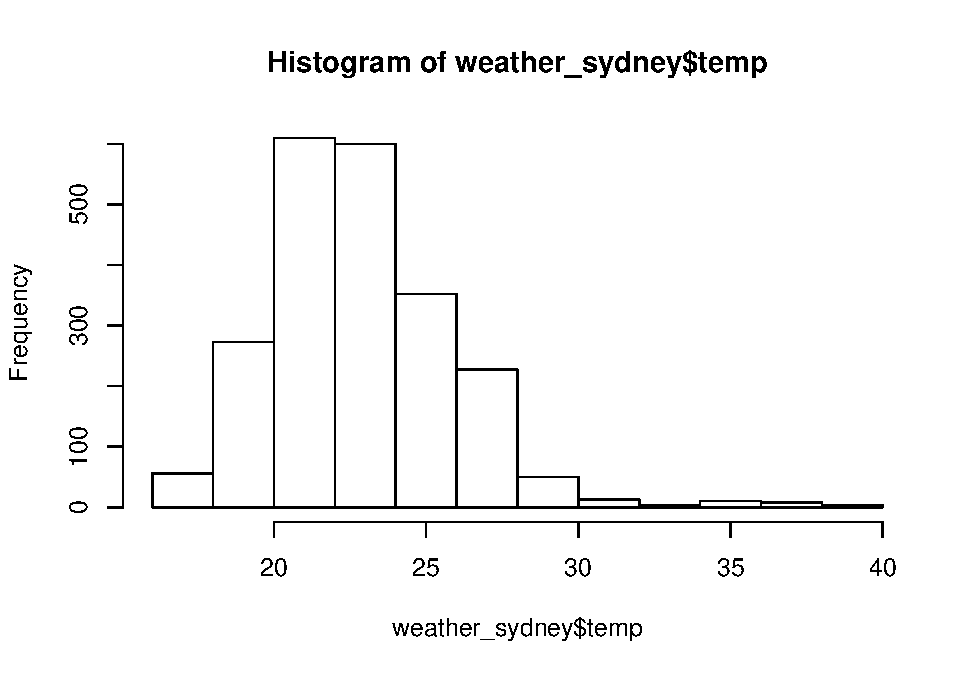
\includegraphics{AT2_template__medium__files/figure-latex/basic histograms-1.pdf}

\begin{Shaded}
\begin{Highlighting}[]
\KeywordTok{hist}\NormalTok{(weather_melbourne}\OperatorTok{$}\NormalTok{temp)}
\end{Highlighting}
\end{Shaded}

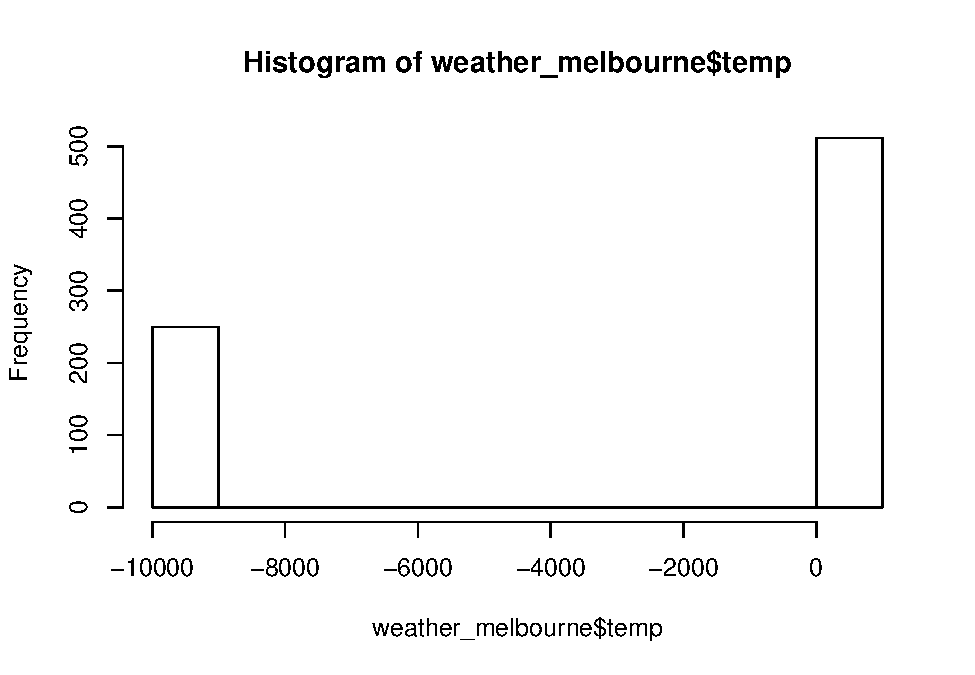
\includegraphics{AT2_template__medium__files/figure-latex/basic histograms-2.pdf}

\begin{Shaded}
\begin{Highlighting}[]
\CommentTok{#this data used to need a lot more cleaning! Previously, you need to remove -9999 values}
\NormalTok{SYD_temp <-}\StringTok{ }\KeywordTok{as.data.frame}\NormalTok{(}\KeywordTok{as.numeric}\NormalTok{(}\KeywordTok{unlist}\NormalTok{(}\KeywordTok{subset}\NormalTok{(weather_sydney, temp }\OperatorTok{>-}\DecValTok{300}\NormalTok{, }\DataTypeTok{select=}\KeywordTok{c}\NormalTok{(}\StringTok{"temp"}\NormalTok{))))) }\CommentTok{#you could also replace these wiht NA, but here we're just going to exclude the missing data}
\KeywordTok{colnames}\NormalTok{(SYD_temp)[}\DecValTok{1}\NormalTok{] <-}\StringTok{ "temp"}
\NormalTok{SYD_temp}\OperatorTok{$}\NormalTok{loc <-}\StringTok{ "SYD"}

\NormalTok{MEL_temp <-}\StringTok{ }\KeywordTok{as.data.frame}\NormalTok{(}\KeywordTok{as.numeric}\NormalTok{(}\KeywordTok{unlist}\NormalTok{(}\KeywordTok{subset}\NormalTok{(weather_melbourne, temp }\OperatorTok{>-}\DecValTok{300}\NormalTok{, }\DataTypeTok{select=}\KeywordTok{c}\NormalTok{(}\StringTok{"temp"}\NormalTok{)))))}
\KeywordTok{colnames}\NormalTok{(MEL_temp)[}\DecValTok{1}\NormalTok{] <-}\StringTok{ "temp"}
\NormalTok{MEL_temp}\OperatorTok{$}\NormalTok{loc <-}\StringTok{ "MEL"}

\NormalTok{temps <-}\StringTok{ }\KeywordTok{rbind}\NormalTok{(SYD_temp, MEL_temp)}
\NormalTok{temps}\OperatorTok{$}\NormalTok{temp <-}\StringTok{ }\KeywordTok{as.numeric}\NormalTok{(temps}\OperatorTok{$}\NormalTok{temp)}
\end{Highlighting}
\end{Shaded}

First off, I did a bit of cleaning (code chunk above). The ggplot
package makes much nicer figures, like that shown in 1, \emph{but}
what's wrong with that figure?

\begin{Shaded}
\begin{Highlighting}[]
\KeywordTok{ggplot}\NormalTok{(temps, }\KeywordTok{aes}\NormalTok{(}\DataTypeTok{x =}\NormalTok{ temp, }\DataTypeTok{fill =}\NormalTok{ loc)) }\OperatorTok{+}\StringTok{ }\KeywordTok{geom_histogram}\NormalTok{(}\DataTypeTok{alpha =} \FloatTok{.5}\NormalTok{, }\DataTypeTok{position =} \StringTok{'identity'}\NormalTok{) }
\end{Highlighting}
\end{Shaded}

\begin{verbatim}
## `stat_bin()` using `bins = 30`. Pick better value with `binwidth`.
\end{verbatim}

\begin{figure}
\centering
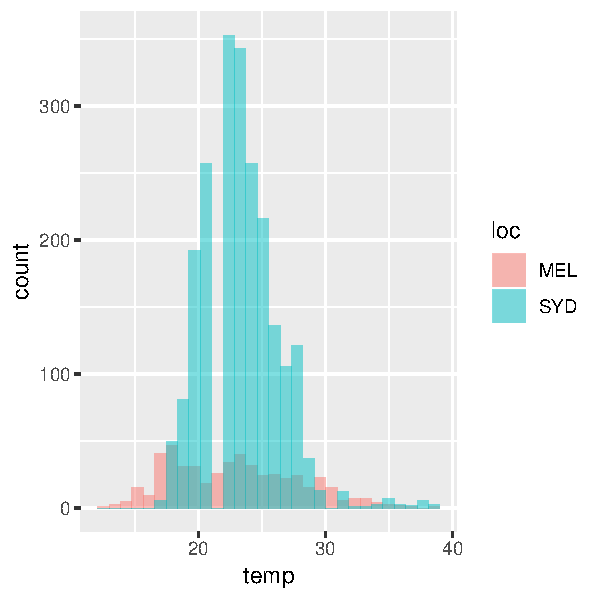
\includegraphics{AT2_template__medium__files/figure-latex/pretty histograms-1.pdf}
\caption{pretty histograms}
\end{figure}

Hm, ok let's try and fix 1 \ldots{}

\begin{Shaded}
\begin{Highlighting}[]
\KeywordTok{ggplot}\NormalTok{(temps, }\KeywordTok{aes}\NormalTok{(}\DataTypeTok{x =}\NormalTok{ temp, }\DataTypeTok{fill =}\NormalTok{ loc)) }\OperatorTok{+}\StringTok{ }\KeywordTok{geom_histogram}\NormalTok{(}\DataTypeTok{alpha =} \FloatTok{.5}\NormalTok{, }\KeywordTok{aes}\NormalTok{(}\DataTypeTok{y =}\NormalTok{ ..density..), }\DataTypeTok{position =} \StringTok{'identity'}\NormalTok{) }\CommentTok{#note use of 'density' because we have unequal temperature counts in each dataset, and this lets us understand the data as a percentage over the period. Alpha is the transparency level.}
\end{Highlighting}
\end{Shaded}

\begin{verbatim}
## `stat_bin()` using `bins = 30`. Pick better value with `binwidth`.
\end{verbatim}

\begin{figure}
\centering
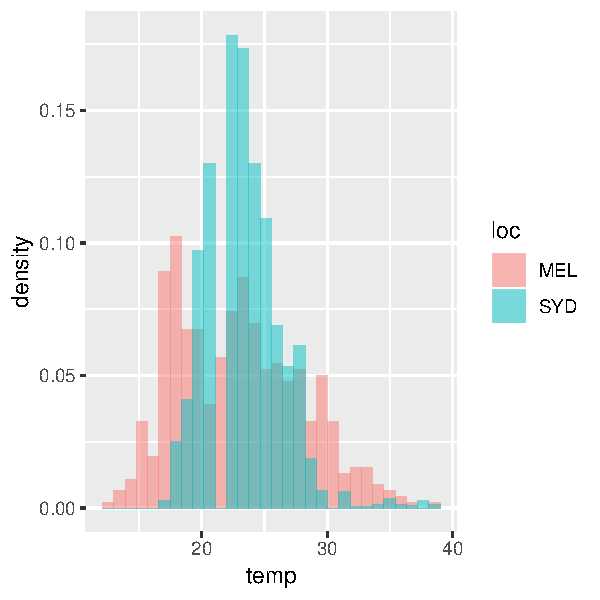
\includegraphics{AT2_template__medium__files/figure-latex/pretty histograms density-1.pdf}
\caption{pretty histograms}
\end{figure}

2 is an improvement. There's another (also simple) way to do this

\begin{Shaded}
\begin{Highlighting}[]
\KeywordTok{histogram}\NormalTok{(}\OperatorTok{~}\StringTok{ }\NormalTok{temp }\OperatorTok{|}\StringTok{ }\NormalTok{loc, }\DataTypeTok{data=}\NormalTok{temps)}
\end{Highlighting}
\end{Shaded}

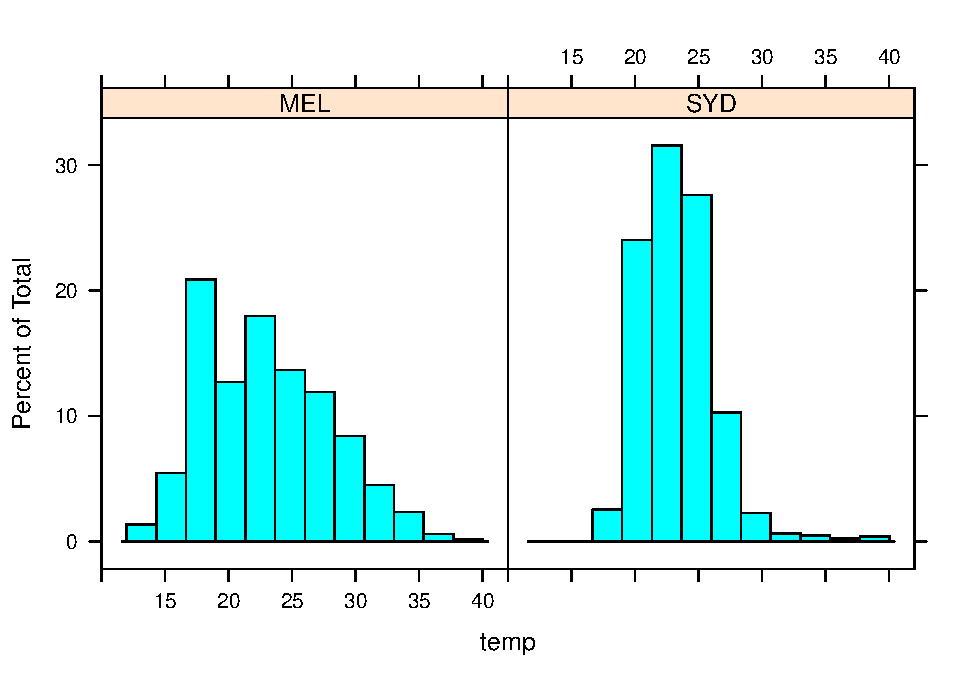
\includegraphics{AT2_template__medium__files/figure-latex/unnamed-chunk-4-1.pdf}

What's wrong with this?

\begin{Shaded}
\begin{Highlighting}[]
\KeywordTok{ggplot}\NormalTok{(temps) }\OperatorTok{+}\StringTok{ }
\StringTok{  }\KeywordTok{geom_bar}\NormalTok{(}\KeywordTok{aes}\NormalTok{(}\DataTypeTok{x =}\NormalTok{ loc, }\DataTypeTok{y =}\NormalTok{ temp, }\DataTypeTok{fill =}\NormalTok{ loc),}
           \DataTypeTok{position =} \StringTok{"dodge"}\NormalTok{, }\DataTypeTok{stat =} \StringTok{"summary"}\NormalTok{, }\DataTypeTok{fun.y =} \StringTok{"mean"}\NormalTok{)}
\end{Highlighting}
\end{Shaded}

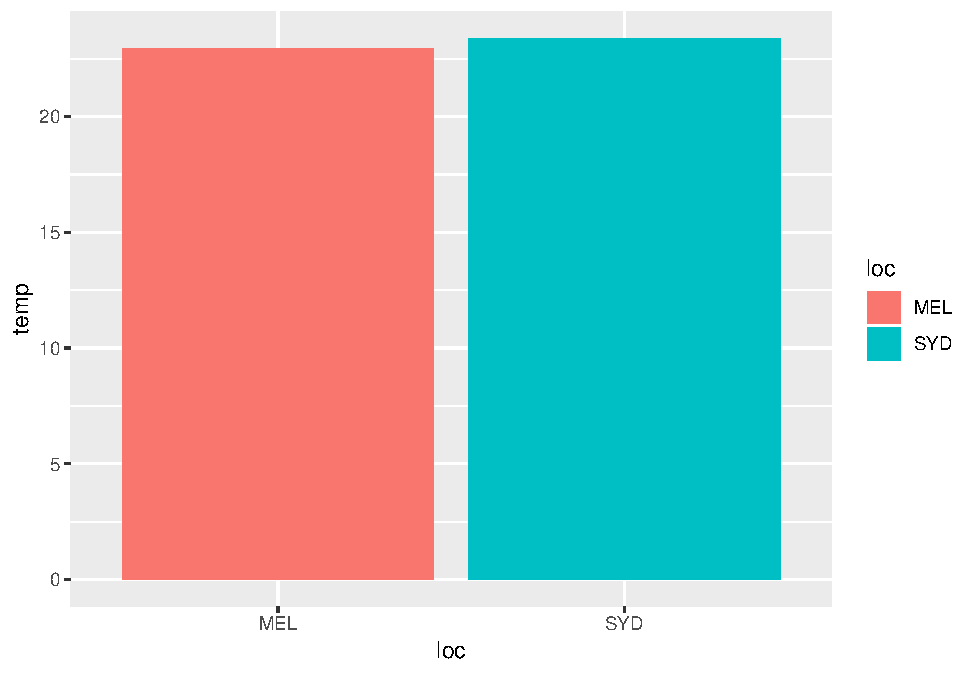
\includegraphics{AT2_template__medium__files/figure-latex/unnamed-chunk-5-1.pdf}

More informative?

\begin{Shaded}
\begin{Highlighting}[]
\KeywordTok{ggplot}\NormalTok{(temps, }\KeywordTok{aes}\NormalTok{(}\DataTypeTok{x=}\NormalTok{loc, }\DataTypeTok{y=}\NormalTok{temp, }\DataTypeTok{fill=}\NormalTok{loc)) }\OperatorTok{+}\StringTok{ }\KeywordTok{geom_boxplot}\NormalTok{() }\OperatorTok{+}
\StringTok{    }\KeywordTok{guides}\NormalTok{(}\DataTypeTok{fill=}\OtherTok{FALSE}\NormalTok{)}\OperatorTok{+}
\StringTok{    }\KeywordTok{stat_summary}\NormalTok{(}\DataTypeTok{fun.y=}\NormalTok{mean, }\DataTypeTok{geom=}\StringTok{"point"}\NormalTok{, }\DataTypeTok{shape=}\DecValTok{5}\NormalTok{, }\DataTypeTok{size=}\DecValTok{4}\NormalTok{)}
\end{Highlighting}
\end{Shaded}

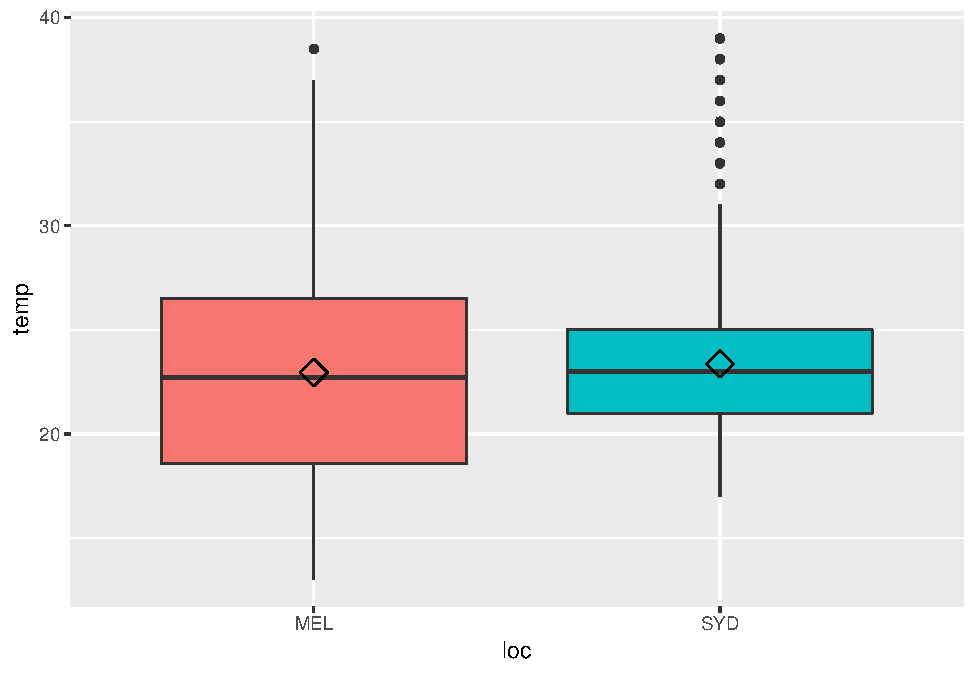
\includegraphics{AT2_template__medium__files/figure-latex/unnamed-chunk-6-1.pdf}

Couple of useful things - let's pull the date out to its own value, and
this time we'll replace missing values (-9999) with NA

\begin{Shaded}
\begin{Highlighting}[]
\KeywordTok{ggplot}\NormalTok{(weather_sydney, }\KeywordTok{aes}\NormalTok{(}\DataTypeTok{x=}\NormalTok{temp, }\DataTypeTok{y=}\NormalTok{dew_pt)) }\OperatorTok{+}
\StringTok{    }\KeywordTok{geom_point}\NormalTok{(}\DataTypeTok{shape=}\DecValTok{1}\NormalTok{)      }\CommentTok{# Use hollow circles}
\end{Highlighting}
\end{Shaded}

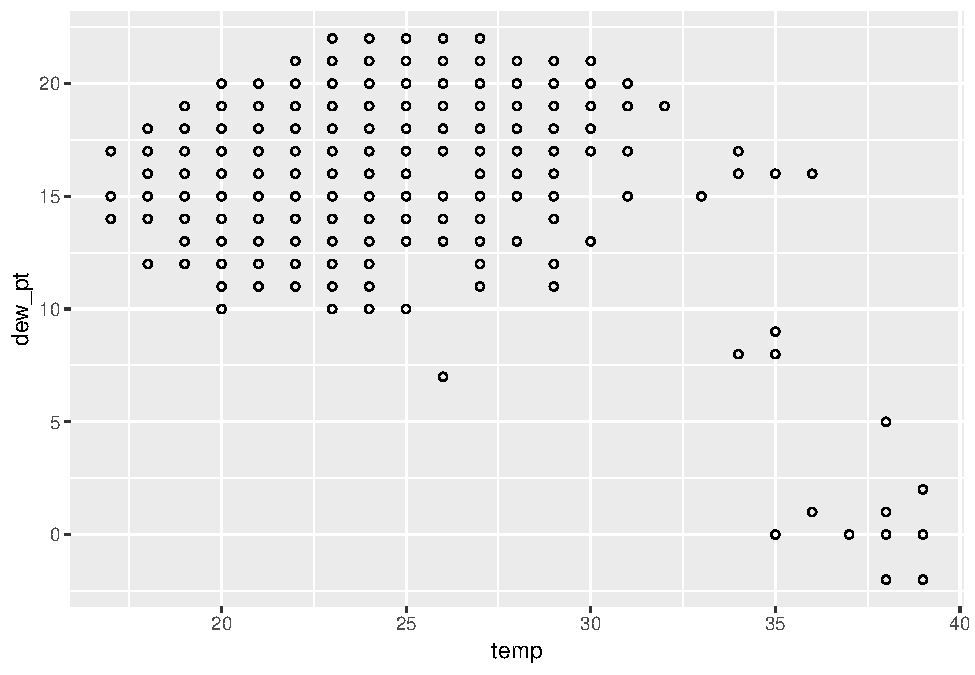
\includegraphics{AT2_template__medium__files/figure-latex/unnamed-chunk-7-1.pdf}

\begin{Shaded}
\begin{Highlighting}[]
\NormalTok{weather_sydney[weather_sydney }\OperatorTok{==}\StringTok{ }\DecValTok{-9999}\NormalTok{] <-}\StringTok{ }\OtherTok{NA}
\NormalTok{weather_sydney}\OperatorTok{$}\NormalTok{date <-}\StringTok{ }\KeywordTok{as.Date}\NormalTok{(weather_sydney}\OperatorTok{$}\NormalTok{date)}

\NormalTok{weather_melbourne[weather_melbourne }\OperatorTok{==}\StringTok{ }\DecValTok{-9999}\NormalTok{] <-}\StringTok{ }\OtherTok{NA}
\NormalTok{weather_melbourne}\OperatorTok{$}\NormalTok{date <-}\StringTok{ }\KeywordTok{as.Date}\NormalTok{(weather_melbourne}\OperatorTok{$}\NormalTok{date)}

\KeywordTok{ggplot}\NormalTok{(weather_sydney, }\KeywordTok{aes}\NormalTok{(}\DataTypeTok{x=}\NormalTok{temp, }\DataTypeTok{y=}\NormalTok{dew_pt)) }\OperatorTok{+}
\StringTok{    }\KeywordTok{geom_point}\NormalTok{(}\DataTypeTok{shape=}\DecValTok{1}\NormalTok{)      }\CommentTok{# Use hollow circles}
\end{Highlighting}
\end{Shaded}

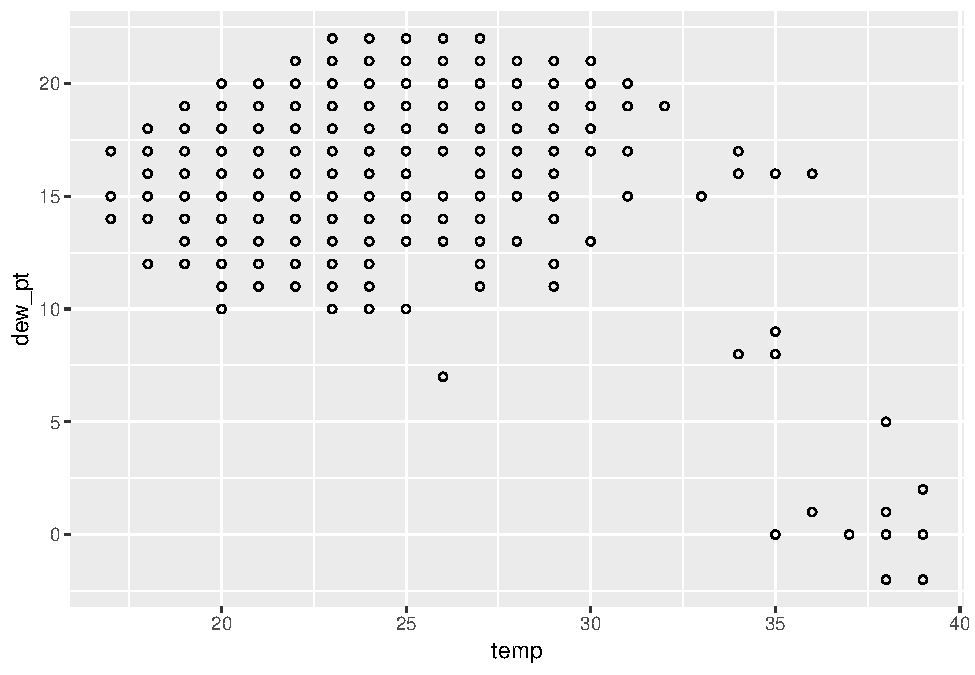
\includegraphics{AT2_template__medium__files/figure-latex/unnamed-chunk-7-2.pdf}

What if we want to explore the relationship between dew\_pt and other
features
\url{https://support.office.com/en-us/article/Present-your-data-in-a-scatter-chart-or-a-line-chart-4570a80f-599a-4d6b-a155-104a9018b86e}

One way you might be tempted to do this\ldots{}

\begin{Shaded}
\begin{Highlighting}[]
\NormalTok{bad_example <-}\StringTok{ }\KeywordTok{subset}\NormalTok{(weather_sydney, }\OperatorTok{!}\KeywordTok{is.na}\NormalTok{(hum), }\DataTypeTok{select=}\KeywordTok{c}\NormalTok{(}\StringTok{"hum"}\NormalTok{, }\StringTok{"dew_pt"}\NormalTok{,}\StringTok{"date"}\NormalTok{))}
\NormalTok{bad_example[}\KeywordTok{c}\NormalTok{(}\StringTok{"hum"}\NormalTok{,}\StringTok{"dew_pt"}\NormalTok{)] <-}\StringTok{ }\KeywordTok{lapply}\NormalTok{(bad_example[}\KeywordTok{c}\NormalTok{(}\StringTok{"hum"}\NormalTok{,}\StringTok{"dew_pt"}\NormalTok{)],as.numeric)}

\NormalTok{bad_example <-}\StringTok{ }\KeywordTok{aggregate}\NormalTok{(. }\OperatorTok{~}\StringTok{ }\NormalTok{date, bad_example, }\DataTypeTok{FUN=}\NormalTok{mean)}

\CommentTok{#convert to long}
\NormalTok{bad_example <-}\StringTok{ }\KeywordTok{melt}\NormalTok{(bad_example, }\DataTypeTok{id.vars =} \KeywordTok{c}\NormalTok{(}\StringTok{"date"}\NormalTok{))}

\KeywordTok{ggplot}\NormalTok{(}\DataTypeTok{data=}\NormalTok{bad_example, }\KeywordTok{aes}\NormalTok{(}\DataTypeTok{x=}\NormalTok{date, }\DataTypeTok{y=}\NormalTok{value, }\DataTypeTok{group=}\NormalTok{variable, }\DataTypeTok{colour=}\NormalTok{variable)) }\OperatorTok{+}
\StringTok{    }\KeywordTok{geom_line}\NormalTok{() }\OperatorTok{+}
\StringTok{    }\KeywordTok{geom_point}\NormalTok{()}
\end{Highlighting}
\end{Shaded}

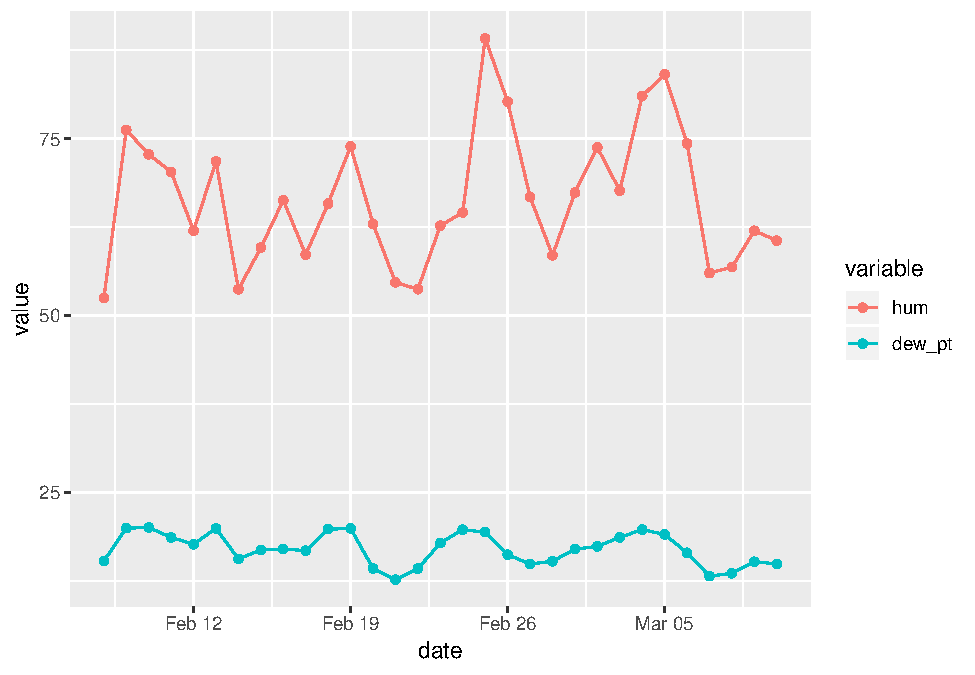
\includegraphics{AT2_template__medium__files/figure-latex/unnamed-chunk-8-1.pdf}

\begin{Shaded}
\begin{Highlighting}[]
\CommentTok{#Is date an important variable in this analysis? Does the scaling of the data gives us the best available insight into relationships of paired values? Is the use of a line to join datapoints appropriate given missing data?}
\end{Highlighting}
\end{Shaded}

A better way?

\begin{Shaded}
\begin{Highlighting}[]
\KeywordTok{ggplot}\NormalTok{(weather_sydney, }\KeywordTok{aes}\NormalTok{(}\DataTypeTok{x=}\NormalTok{hum, }\DataTypeTok{y=}\NormalTok{dew_pt)) }\OperatorTok{+}
\StringTok{    }\KeywordTok{geom_point}\NormalTok{(}\DataTypeTok{shape=}\DecValTok{1}\NormalTok{)      }\CommentTok{# Use hollow circles}
\end{Highlighting}
\end{Shaded}

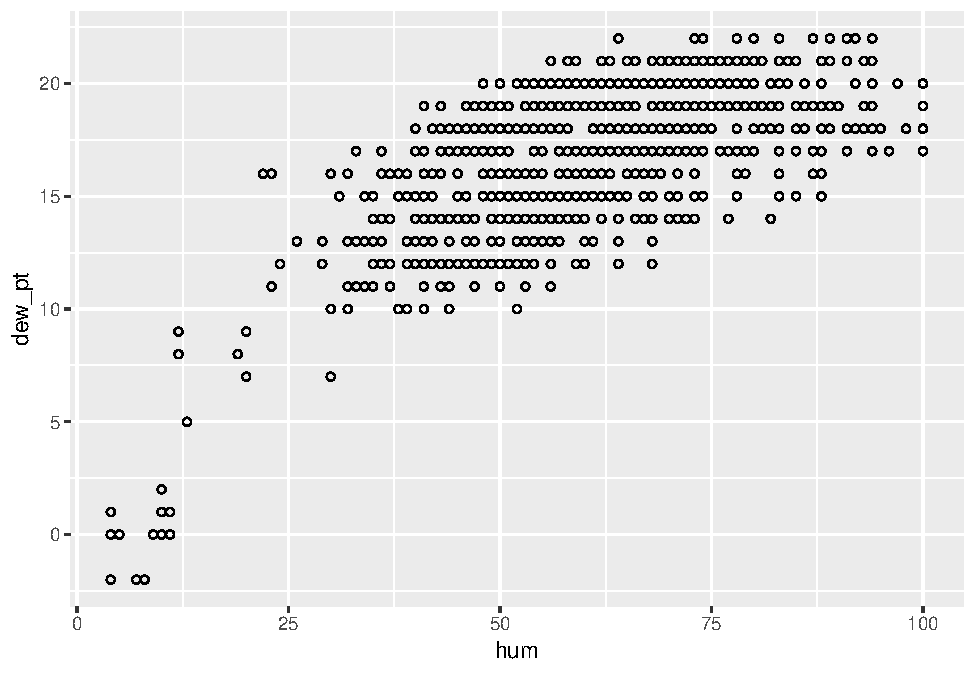
\includegraphics{AT2_template__medium__files/figure-latex/unnamed-chunk-9-1.pdf}

\begin{Shaded}
\begin{Highlighting}[]
\KeywordTok{cor.test}\NormalTok{(}\KeywordTok{as.numeric}\NormalTok{(weather_sydney}\OperatorTok{$}\NormalTok{hum),}\KeywordTok{as.numeric}\NormalTok{(weather_sydney}\OperatorTok{$}\NormalTok{dew_pt))}
\end{Highlighting}
\end{Shaded}

\begin{verbatim}
## 
##  Pearson's product-moment correlation
## 
## data:  as.numeric(weather_sydney$hum) and as.numeric(weather_sydney$dew_pt)
## t = 40.31, df = 2204, p-value < 2.2e-16
## alternative hypothesis: true correlation is not equal to 0
## 95 percent confidence interval:
##  0.6267465 0.6748281
## sample estimates:
##       cor 
## 0.6514409
\end{verbatim}

Of course, you don't have to just display the correlation, you can
**\emph{output the coefficient in-line with code: 0.6514409}*

Ok what if we want to look at how weather varies over time and place?

\begin{Shaded}
\begin{Highlighting}[]
\NormalTok{weather_sydney}\OperatorTok{$}\NormalTok{loc <-}\StringTok{ "Sydney"}
\NormalTok{weather_melbourne}\OperatorTok{$}\NormalTok{loc <-}\StringTok{ "Melbourne"}
\end{Highlighting}
\end{Shaded}

\begin{Shaded}
\begin{Highlighting}[]
\NormalTok{weather <-}\StringTok{ }\KeywordTok{rbind}\NormalTok{(weather_sydney[}\KeywordTok{c}\NormalTok{(}\StringTok{"temp"}\NormalTok{,}\StringTok{"dew_pt"}\NormalTok{,}\StringTok{"hum"}\NormalTok{,}\StringTok{"wind_spd"}\NormalTok{,}\StringTok{"precip_total"}\NormalTok{,}\StringTok{"cond"}\NormalTok{,}\StringTok{"date"}\NormalTok{,}\StringTok{"loc"}\NormalTok{)],weather_melbourne[}\KeywordTok{c}\NormalTok{(}\StringTok{"temp"}\NormalTok{,}\StringTok{"dew_pt"}\NormalTok{,}\StringTok{"hum"}\NormalTok{,}\StringTok{"wind_spd"}\NormalTok{,}\StringTok{"precip_total"}\NormalTok{,}\StringTok{"cond"}\NormalTok{,}\StringTok{"date"}\NormalTok{,}\StringTok{"loc"}\NormalTok{)])}
\NormalTok{weather}\OperatorTok{$}\NormalTok{month <-}\StringTok{ }\KeywordTok{format}\NormalTok{(}\KeywordTok{as.Date}\NormalTok{(weather}\OperatorTok{$}\NormalTok{date), }\StringTok{"%m"}\NormalTok{)}

\KeywordTok{ggplot}\NormalTok{(weather, }\KeywordTok{aes}\NormalTok{(}\DataTypeTok{x=}\NormalTok{month, }\DataTypeTok{y=}\NormalTok{temp, }\DataTypeTok{fill=}\NormalTok{loc)) }\OperatorTok{+}\StringTok{ }\KeywordTok{geom_boxplot}\NormalTok{() }\OperatorTok{+}
\StringTok{    }\KeywordTok{guides}\NormalTok{(}\DataTypeTok{fill=}\OtherTok{FALSE}\NormalTok{) }\OperatorTok{+}
\StringTok{    }\KeywordTok{stat_summary}\NormalTok{(}\DataTypeTok{fun.y=}\NormalTok{mean, }\DataTypeTok{geom=}\StringTok{"point"}\NormalTok{, }\DataTypeTok{shape=}\DecValTok{5}\NormalTok{, }\DataTypeTok{size=}\DecValTok{4}\NormalTok{) }\OperatorTok{+}
\StringTok{    }\KeywordTok{facet_wrap}\NormalTok{(}\OperatorTok{~}\NormalTok{loc)}
\end{Highlighting}
\end{Shaded}

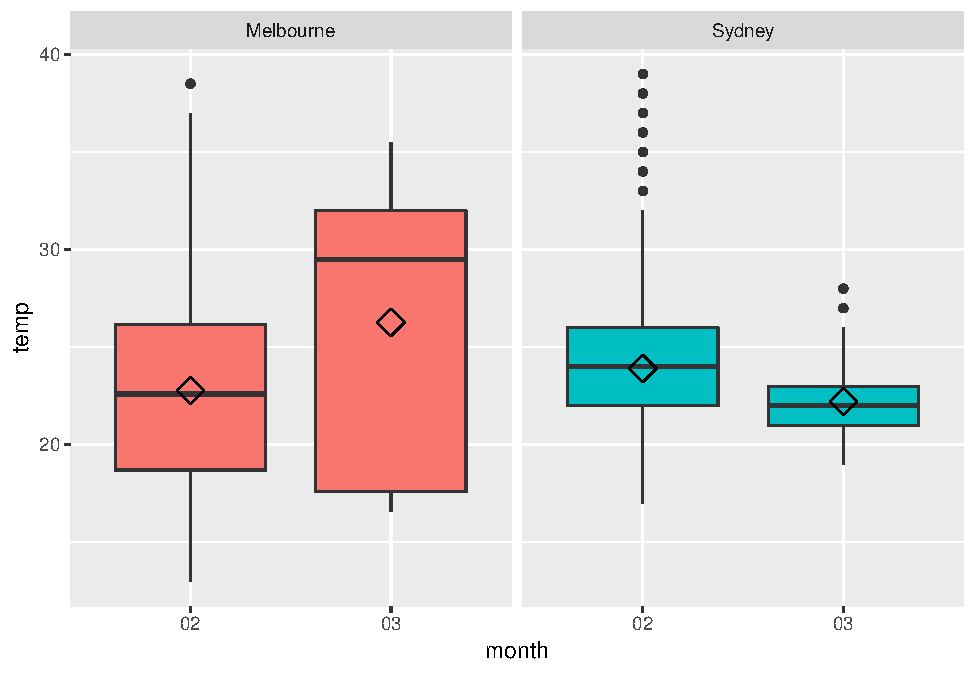
\includegraphics{AT2_template__medium__files/figure-latex/unnamed-chunk-11-1.pdf}

Or at how weather events vary by place

\begin{Shaded}
\begin{Highlighting}[]
\CommentTok{#unique(weather$Events)}
\KeywordTok{unique}\NormalTok{(weather}\OperatorTok{$}\NormalTok{cond)}
\end{Highlighting}
\end{Shaded}

\begin{verbatim}
##  [1] "Partly Cloudy"                "Clear"                       
##  [3] ""                             "Mostly Cloudy"               
##  [5] "Scattered Clouds"             "Haze"                        
##  [7] "Thunderstorm"                 "Light Rain Showers"          
##  [9] "Light Thunderstorms and Rain" "Light Rain"                  
## [11] "Overcast"                     "Unknown"                     
## [13] "Rain Showers"                 "Light Drizzle"               
## [15] "Drizzle"                      "Heavy Rain Showers"          
## [17] "Rain"                         NA
\end{verbatim}

\begin{Shaded}
\begin{Highlighting}[]
\KeywordTok{table}\NormalTok{(weather}\OperatorTok{$}\NormalTok{cond,weather}\OperatorTok{$}\NormalTok{loc)}
\end{Highlighting}
\end{Shaded}

\begin{verbatim}
##                               
##                                Melbourne Sydney
##                                        0    470
##   Clear                                0    285
##   Drizzle                              0      3
##   Haze                                 0     63
##   Heavy Rain Showers                   0      2
##   Light Drizzle                        0     11
##   Light Rain                           0     40
##   Light Rain Showers                   0     72
##   Light Thunderstorms and Rain         0      5
##   Mostly Cloudy                        0    591
##   Overcast                             0     27
##   Partly Cloudy                        0    362
##   Rain                                 0     10
##   Rain Showers                         0     13
##   Scattered Clouds                     0    247
##   Thunderstorm                         0      1
##   Unknown                              0      4
\end{verbatim}

\begin{Shaded}
\begin{Highlighting}[]
\NormalTok{weather_con <-}\StringTok{ }\KeywordTok{unique}\NormalTok{(}\KeywordTok{subset}\NormalTok{(weather,}\DataTypeTok{select=}\KeywordTok{c}\NormalTok{(}\StringTok{"cond"}\NormalTok{,}\StringTok{"date"}\NormalTok{,}\StringTok{"loc"}\NormalTok{)))}

\KeywordTok{ggplot}\NormalTok{(}\DataTypeTok{data=}\NormalTok{weather_con, }\KeywordTok{aes}\NormalTok{(}\DataTypeTok{x=}\NormalTok{cond, }\DataTypeTok{fill =}\NormalTok{ loc)) }\OperatorTok{+}
\StringTok{    }\KeywordTok{geom_bar}\NormalTok{(}\DataTypeTok{position=}\KeywordTok{position_dodge}\NormalTok{()) }\OperatorTok{+}
\StringTok{    }\KeywordTok{theme}\NormalTok{(}\DataTypeTok{axis.text.x =} \KeywordTok{element_text}\NormalTok{(}\DataTypeTok{angle =} \DecValTok{90}\NormalTok{, }\DataTypeTok{vjust =} \FloatTok{.5}\NormalTok{, }\DataTypeTok{hjust =} \DecValTok{1}\NormalTok{))}
\end{Highlighting}
\end{Shaded}

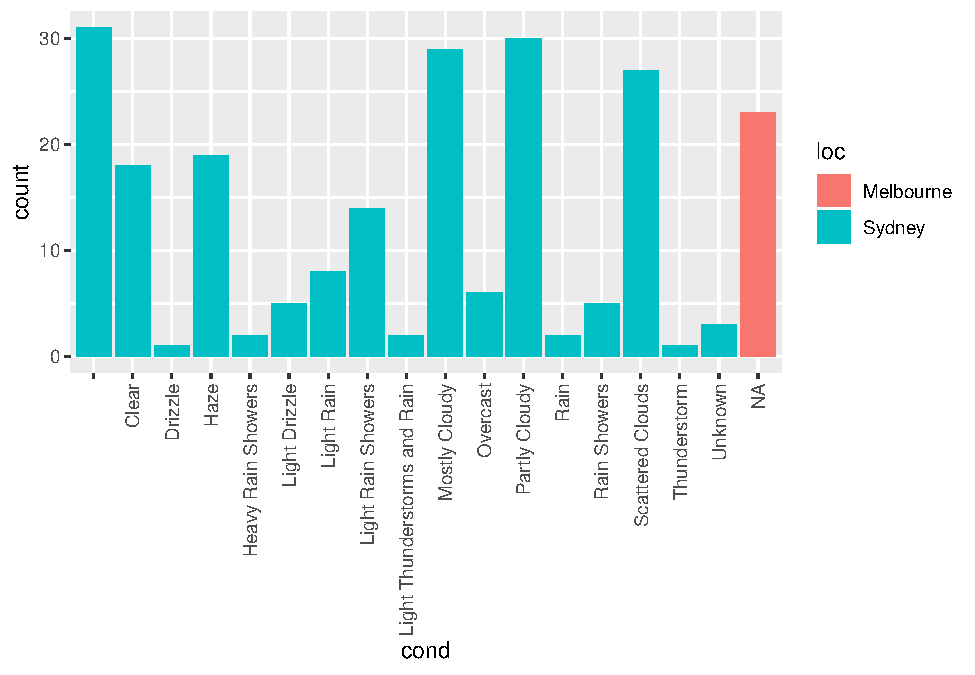
\includegraphics{AT2_template__medium__files/figure-latex/unnamed-chunk-12-1.pdf}

\begin{Shaded}
\begin{Highlighting}[]
\CommentTok{#weather_con <- unique(subset(weather,select=c("Events","DateUTC","loc")))}
\CommentTok{#ggplot(data=weather_con, aes(x=Events, fill = loc)) +}
 \CommentTok{#   geom_bar(position=position_dodge()) +}
    \CommentTok{#scale_y_continuous(labels=scales::percent) +}
  \CommentTok{#  theme(axis.text.x = element_text(angle = 90, vjust = .5, hjust = 1))}
\end{Highlighting}
\end{Shaded}

We've often seen students refer to `average mood'. Sometimes this might
make sense, but this is an analogous example\ldots{}

\begin{Shaded}
\begin{Highlighting}[]
\CommentTok{#let's take the weather event data, and code it from best ('no event') to worst ('snow')}
\NormalTok{weather_con}\OperatorTok{$}\NormalTok{cond[weather_con}\OperatorTok{$}\NormalTok{cond}\OperatorTok{==}\StringTok{"Clear"}\NormalTok{] <-}\StringTok{ }\DecValTok{7}
\NormalTok{weather_con}\OperatorTok{$}\NormalTok{cond[weather_con}\OperatorTok{$}\NormalTok{cond}\OperatorTok{==}\StringTok{""}\NormalTok{] <-}\StringTok{ }\DecValTok{6}
\NormalTok{weather_con}\OperatorTok{$}\NormalTok{cond[weather_con}\OperatorTok{$}\NormalTok{cond}\OperatorTok{==}\StringTok{"Mostly Cloudy"}\NormalTok{] <-}\StringTok{ }\DecValTok{5}
\NormalTok{weather_con}\OperatorTok{$}\NormalTok{cond[weather_con}\OperatorTok{$}\NormalTok{cond}\OperatorTok{==}\StringTok{"Light Rain Showers"}\NormalTok{] <-}\StringTok{ }\DecValTok{4}
\NormalTok{weather_con}\OperatorTok{$}\NormalTok{cond[weather_con}\OperatorTok{$}\NormalTok{cond}\OperatorTok{==}\StringTok{"Light Thunderstorms and Rain"}\NormalTok{] <-}\StringTok{ }\DecValTok{3}
\NormalTok{weather_con}\OperatorTok{$}\NormalTok{cond[weather_con}\OperatorTok{$}\NormalTok{cond}\OperatorTok{==}\StringTok{"Heavy Rain Showers"}\NormalTok{] <-}\StringTok{ }\DecValTok{2}
\NormalTok{weather_con}\OperatorTok{$}\NormalTok{cond[weather_con}\OperatorTok{$}\NormalTok{cond}\OperatorTok{==}\StringTok{"Thunderstorm"}\NormalTok{] <-}\StringTok{ }\DecValTok{1}

\NormalTok{weather_con}\OperatorTok{$}\NormalTok{cond <-}\StringTok{ }\KeywordTok{as.numeric}\NormalTok{(weather_con}\OperatorTok{$}\NormalTok{cond)}

\KeywordTok{ggplot}\NormalTok{(weather_con, }\KeywordTok{aes}\NormalTok{(}\DataTypeTok{x =}\NormalTok{ loc, }\DataTypeTok{y =}\NormalTok{ cond, }\DataTypeTok{fill=}\NormalTok{loc)) }\OperatorTok{+}\StringTok{ }\KeywordTok{geom_boxplot}\NormalTok{() }\OperatorTok{+}
\StringTok{    }\KeywordTok{stat_summary}\NormalTok{(}\DataTypeTok{fun.y=}\NormalTok{mean, }\DataTypeTok{geom=}\StringTok{"point"}\NormalTok{, }\DataTypeTok{shape=}\DecValTok{5}\NormalTok{, }\DataTypeTok{size=}\DecValTok{4}\NormalTok{)}
\end{Highlighting}
\end{Shaded}

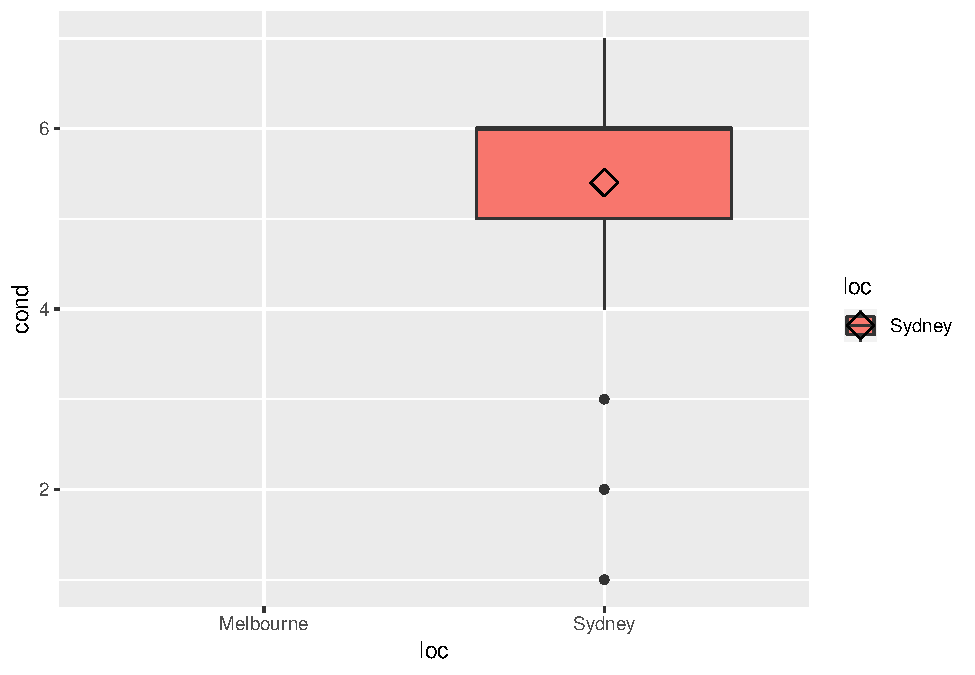
\includegraphics{AT2_template__medium__files/figure-latex/unnamed-chunk-13-1.pdf}

\hypertarget{findings-and-conclusions}{%
\section{Findings and Conclusions}\label{findings-and-conclusions}}

\textless what conclusions did you come to as a result of the analysis
of your data and of the group's data.\\
Criterion 2: Justifies the analysis of the obtained data, including
quality issues, to draw conclusions in a professional and engaging
manner.\textgreater{}

\hypertarget{discussion}{%
\section{Discussion}\label{discussion}}

\textless discuss aspects of the process that you see as important. For
example, what difficulties did you encounter; how could you avoid
problems if you did it again; etc\textgreater{}

Your `justification' and evaluation of your approach is likely to go in
this section, but may also be threaded through the preceding sections.
This includes Criterion 3: Identifies, contextualises, and reflects on
the ethical, privacy, and legal issues relevant to the collection and
analysis of personal data of self and others. \textgreater{}

\hypertarget{reflection}{%
\section{Reflection}\label{reflection}}

\textless General reflection on what you learnt during this task. What
are you unsure about? What would you do differently if you had to do it
all again?\\
Criteria 4: Connects the individual experience of this QS project to the
practice of data science (and the preceding three criteria).
\textgreater{}

\hypertarget{other}{%
\section{Other}\label{other}}

If you are submitting any additional materials, such as short multimedia
presentations or visualisations (such as Prezi, or voice-over
video/screen capture, etc), they probably can't be submitted through
UTSOnline so you will need to arrange some other process such as posting
on YouTube or elsewhere, or handing in a memory stick or CD/DVD. Please
ensure that additional material like this is accessible to the markers
(test this by accessing it through someone else's computer) and avoid
any restrictive or proprietary software constraints. Remember to check
any inculded web links!

Diagrams, figures, charts and illustrations must be labelled, and
explained, and must be referred to from somewhere in the report. If
drawn from another source, then the source must be provided.

\hypertarget{references}{%
\section{References}\label{references}}

\begin{Shaded}
\begin{Highlighting}[]
  \KeywordTok{write.bibtex}\NormalTok{(}\DataTypeTok{file=}\StringTok{"references.bib"}\NormalTok{)}
\end{Highlighting}
\end{Shaded}

\hypertarget{refs}{}
\leavevmode\hypertarget{ref-Boettiger_2017}{}%
Boettiger, C. (2017). \emph{Knitcitations: Citations for 'knitr'
markdown files}. Retrieved from
\url{https://CRAN.R-project.org/package=knitcitations}

\leavevmode\hypertarget{ref-Halpern_2006}{}%
Halpern, B.S., Regan, H.M., Possingham, H.P. \& McCarthy, M.A. (2006).
Accounting for uncertainty in marine reserve design. \emph{Ecology
Letters}, \textbf{9}, 2--11. Retrieved from
\url{https://doi.org/10.1111/j.1461-0248.2005.00827.x}

\leavevmode\hypertarget{ref-Keil_2012}{}%
Keil, P., Belmaker, J., Wilson, A.M., Unitt, P. \& Jetz, W. (2012).
Downscaling of species distribution models:
\textless U+2028\textgreater a hierarchical approach (R. Freckleton,
Ed.). \emph{Methods in Ecology and Evolution}, \textbf{4}, 82--94.
Retrieved from \url{https://doi.org/10.1111/j.2041-210x.2012.00264.x}

\leavevmode\hypertarget{ref-greycite380215}{}%
Knight, S. \& Shum, S.B. (2020). Artificial intelligence holds great
potential for both students and teachers \&ndash; but only if used
wisely. \emph{The Conversation}. Retrieved from
\url{https://theconversation.com/artificial-intelligence-holds-great-potential-for-both-students-and-teachers-but-only-if-used-wisely-81024}

\leavevmode\hypertarget{ref-R_Core_Team_2018}{}%
R Core Team. (2018). \emph{R: A language and environment for statistical
computing}. R Foundation for Statistical Computing, Vienna, Austria.
Retrieved from \url{https://www.R-project.org/}


\end{document}
